% main.tex
\documentclass{article}

\usepackage[pdfauthor={CoderDojo Linz},
            pdftitle={Bubble-sorter-in-Scratch}]
            {hyperref}



\newcommand{\footertitle}{Bubble sorter in Scratch}
% settings.tex
\usepackage[
    a4paper, 
    top=2cm,
    left=1cm,
    right=1cm,
    bottom=2cm
]{geometry}

\usepackage{fontspec}
\usepackage{graphicx}
\usepackage{hyperref}
\usepackage{fancyhdr}
\usepackage[ngerman]{babel}
\usepackage{wrapfig}
\usepackage{enumitem}
\usepackage{titlesec} 
\usepackage{ragged2e}
\usepackage{tcolorbox}
\usepackage{array}
\usepackage[table]{xcolor}
\usepackage{fontawesome5}

\setmainfont{Carlito}

% Fancyhdr setup
\fancypagestyle{defaultpagestyle}{
    \fancyhf{} % Clear all headers and footers
    \fancyhead[C]{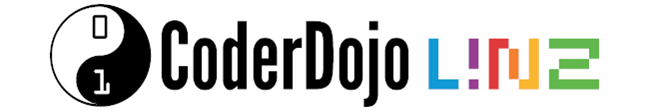
\includegraphics[width=5cm]{../../CoderDojo_Logo.png}} 
    \renewcommand{\headrulewidth}{0pt} % Remove header line
    \renewcommand{\footrulewidth}{0pt} % Remove footer line
    \fancyfoot[L]{\footertitle}
    \fancyfoot[R]{Seite \thepage} % Right footer with page number
}

\newcommand{\SectionDesign}[4]{
    \noindent
    \csname #1*\endcsname{\textcolor[HTML]{1E90FF}{\fontsize{#2pt}{#3pt}\selectfont #4}}
}

\newcommand{\TextAndImage}[5][{}]{
    \fontsize{11pt}{16pt}\selectfont
    \noindent
    \begin{minipage}[c]{#4\textwidth}
    \RaggedRight
    #2 % First parameter: text
    \end{minipage}
    \hfill
    \begin{minipage}[c]{#5\textwidth}
    \includegraphics[width=\textwidth, #1]{#3} % Second parameter: image file name
    \end{minipage}
}

\newcommand{\ImageAndText}[2]{
    \fontsize{16pt}{24pt}\selectfont
    \noindent
    \begin{minipage}[c]{0.65\textwidth}
        \includegraphics[width=\textwidth]{#1} % Second parameter: image file name
    \end{minipage}
    \hfill % Fills the space between the minipages
    \begin{minipage}[c]{0.25\textwidth}
        \centering
        #2 % First parameter: text
    \end{minipage}
}

\newcommand{\TextDesign}[1]{
    \fontsize{11pt}{16pt}\selectfont
    \noindent
    \RaggedRight
    #1 % First parameter: text
}
\graphicspath{{images/}}

\begin{document}
    \pagestyle{defaultpagestyle}

    \SectionDesign{section}{24}{24}{\textbf{Bubble Sorter mit Scratch}}
    \vspace{1cm}
     
    \ImageAndText{MainPic.png}{
    \centering
    Heute programmieren wir eine herausfordernde Scratch Übung namens Bubble Sorter. Hierbei kannst du deine Scratch Kenntnisse verbessern.
    }{0.6}{0.3}{16}{24}
    
    \vspace{2cm}
    \SectionDesign{subsection}{18}{24}{\textbf{Ziel der Übung}}
    \vspace{0.5cm}

    \TextDesign{
    Heute wollen wir gemeinsam einen Bubble Sorter basteln, hierbei geht es darum den Algorithmus zu verstehen, mit Klonen zu Arbeiten und dich selber etwas heraus zu fordern.Du solltest für diese Übung schon ein wenig Programmiererfahrung mit einer Block Programmiersprache wie \textit{Scratch} oder \textit{Snap!} haben. }


    \vspace{1cm}
    \SectionDesign{subsection}{18}{24}{\textbf{Start}}
    \vspace{0.5cm}

    \TextDesign{
    Du brauchst für diese Übung keine spezielle Software auf deinem Computer zu installieren. Scratch kannst du auch im Web-browser verwenden. Um los zu legen müssen wir als erstes unsere Figuren und den Hintergrund fest legen. Wir brauchen dafür Bälle und natürlich ein Gefäß dafür. Eine Figur die mit dem Benutzer spricht und einen schönen Hintergrund. In den Unteren Links kannst du dir deine Figuren runter laden}

\begin{itemize}
        \item \url{https://meet.coderdojo.net/biber-sprite}
         \item \url{https://meet.coderdojo.net/ball-sprite}
        \item \url{https://meet.coderdojo.net/behälter-sprite}
 
    \end{itemize}
    
     % NEWPAGE
    \newpage
    
 
   
\SectionDesign{subsection}{18}{24}{\textbf{Behälter}}
   \vspace{0.5cm}

   
\TextAndImage{
   Wir fangen an mit unseren Gefäßen für die Bälle. Den lila Block brauchen wir dafür das die Gefäße nicht vor den Bällen sind und sie verdecken. Danach legen wir fixe y und x Koordinaten fest. Die Variable \textit{Position Behälter}. Jedes mal wenn diese Variable erhöht wird wird eine neue Position festgelegt. Dafür brauchen wir unsere Formel unter den Block \textit{Wenn ich als Klone entstehe}. Das kannst du J Jetzt schon mal
    }{CupBlöcke.png}{0.4}{0.5}{11}{16}



          \vspace{0.5cm}
               \TextAndImage{
Am Anfang bekommst du zwei Blöcke, die du brauchen wirst einfach mal zum abtippen! Damit kannst du einfach anfangen. Den ersten Block brauchen wir zum entfernen eines Zeichens am Index i.
    }{ZeichenEntfernen.png}{0.4}{0.4}{11}{16}

          \vspace{0.5cm}
               \TextAndImage{
Das ist der zweite Block, denn du abtippen musst! Dieser fügt am Anfang wider ein beliebiges Zeichen hinzu. 
    }{ZeichenHinzufügen.png}{0.4}{0.4}{11}{16}

   \vspace{0.5cm}

 \TextAndImage{
Hier fragen wir den Benutzer in welchen Behälter er den Ball geben möchte. Du kannst ihn mal nachbauen und schauen was raus kommt! Probier ruhig alles mögliche ein zu geben fällt dir was auf? 
    }{ZielGefäß1.png}{0.4}{0.4}{11}{16}
    
    \vspace{0.5cm}

     \TextAndImage{
Falls du den Fehler nicht gefunden hast ist es nicht schlimm. Wir dürfen natürlich wie bei unseren ersten Block nur Zahlen zwischen 1 und 3 eingeben ,weil wir ja nur 3 Behälter haben. Das machen wir mit einen "Falls" Block. Probiere dich jetzt wider durch und überlege was noch schief gehen könnte! 
    }{ZielGefäß2.png}{0.4}{0.4}{11}{16}

        \vspace{0.5cm}

     \TextAndImage{
Richtig! Falls du den Fehler nicht gefunden hast, kein Problem! Wir müssen natürlich schauen das die Farbe darunter stimmt das machen wir wieder mit einen "Falls" Block. Einen Fehler haben wir noch. Kleiner Tipp: Überlege in welchen Behälter wir Kugeln hinzu fügen können! Darunter siehst du die Verschachtelung nochmal groß
    }{ZielGefäß3.png}{0.4}{0.6}{11}{16}

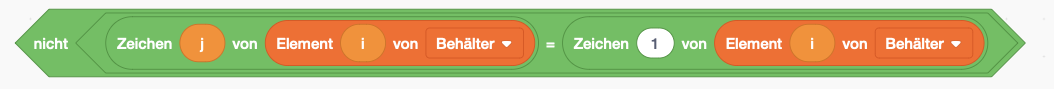
\includegraphics[width=20cm]{FrageL.png}

\vspace{0.5cm}

     \TextAndImage{
Genau! Wir müssen natürlich noch prüfen, ob der Behälter nicht mehr als 3 Kugeln beinhaltet! 
    }{ZielGefäß4.png}{0.4}{0.6}{11}{16}

    
 \vspace{0.5cm}

     \TextAndImage{
Als Erstes fangen wir damit an den Benutzer zu fragen. Von wo er den Block überhaupt nehmen möchte. Du findest auf den Bildern auch immer Kommentare die dir den Block nochmals erklären. Das machen wir hier mit einer Frage und einer Variable worin wir die Antwort speichern. Probiere es doch mal aus. Findest du den Fehler?
    }{FrageQuell1.png}{0.4}{0.4}{11}{16}

     \vspace{0.5cm}

     
     \TextAndImage{
Richtig! Falls du den Fehler nicht gefunden hast ist das nicht schlimm! Wir dürfen natürlich nur Zahlen zwischen 1 und 3 eingeben, da wir nur 3 Behälter haben. Das überprüfen wir  mt einen "Falls" Block. Probiere und überlege wider findest du noch einen Fehler?
    }{FrageQuell2.png}{0.4}{0.4}{11}{16}


     \vspace{0.5cm}

     
     \TextAndImage{
Genau! Falls du den Fehler nicht gefunden hast, ist das nicht schlimm! Wir können den Ball nicht aus einen leeren Behälter nehmen! Das überprüfen wir wieder mit einen "Falls" Block. Eine Hürde gibt es aber noch!
    }{FrageQuell3.png}{0.4}{0.4}{11}{16}


\vspace{0.5cm}

     
     \TextAndImage{
Hier musst du prüfen ob der Benutzer bereits gewonnen hat. Hier prüfen wir am Anfang in einer Schleife ob ein Behälter leer ist wenn ja setzen wir unsere Variable "Leer" auf 1 sodass der Rest voll sein muss. Danach überprüfen wir ob in den anderen Behältern auch immer nur die gleiche Farbe drinnen ist }{PrüfeObGewonnen.png}{0.4}{0.6}{11}{16}


\vspace{1cm}

   \includegraphics[width=20cm]{PrüfeObGewonnenL.png}
\vspace{1cm}

     \TextAndImage{
Jetzt müssen wir unsere Behälter füllen das machen wir mit diesen Block. Wir haben eine Schleife die 2 mal wiederholt wird um unsere 2 Behälter zu befüllen danach haben wir noch eine Schleife die 3 mal durch geht, da wir 3 Bälle in einen Behälter haben möchten.In dieser bestimmen wir mit einer Zufallszahl die Farbe und entfernen ein Zeichen von der Schlange am Anfang. 
    }{GefäßeFüllen.png}{0.4}{0.6}{11}{16}

\vspace{0.5cm}

\TextAndImage{
Jetzt musst du alles nur noch Zusammen fügen. Die rosa Blöcke sind die, die wir uns selber erstellt haben. Das Kostüm brauchen wir für den Gewinner-Bildschirm. Die Nachricht "Kostüm von Bällen ändern" wird an alle Klone von den Bällen gesendet. Die Schleife und das falls brauchen wir um immer wider zu fragen wenn etwas falsch eingegeben wurde. Jetzt sind wir fast fertig mit unseren Biber-Blöcken.
    }{FertigStellen.png}{0.4}{0.5}{11}{16}

    \vspace{0.5cm}

\TextAndImage{
Mit diesen Block teilen wir unseren Klone Position und Kostüm zu. 
    }{GewinnerKlone.png}{0.4}{0.5}{11}{16}
    
\vspace{0.5cm}
  
\TextAndImage{
Auch bei unseren Ball brauchen wir diesen Block wieder, du musst ihn wieder erstellen und dann einfach abtippen. 
    }{EntferneText.png}{0.4}{0.5}{11}{16}

    \vspace{0.5cm}
  
\TextAndImage{
Hier setzten wir das Kostüm für unseren Ball fest}
{BallKostüm.png}{0.4}{0.5}{11}{16}
    
\vspace{0.5cm}
  
\TextAndImage{
Diesen Block brauchen wir um unsere Bälle zufüllen. Heißt wir setzen fixe Bälle und ändern dann nur die Kostüme.
    }{BälleFüllen.png}{0.4}{0.3}{11}{16}
    
    \vspace{0.5cm}
  
\TextAndImage{
Hier legen wir Positionen und Kostüme für unsere geklonten Bälle fest. }
{BallKlone.png}{0.4}{0.3}{11}{16}


\vspace{0.5cm}
  
\TextAndImage{
Hier haben wir noch drei kleine Code Schnipsel die wir brauchen. Das Erste legt fest, wenn die Flagge gedrückt wird das sich der Ball verstecken soll. Das Zweite zeigt an was gemacht wird, wenn die Nachricht "Kostüm von Bälle ändern" empfangen wird, in diesen Fall wird wieder ein Block von uns aufgerufen. Der Dritte zeigt was passiert, wenn die Nachricht "Bälle erstellen" empfangen wird, hier wird ebenfalls ein Block von uns aufgerufen. }
{CodeSchnipsel.png}{0.4}{0.3}{11}{16}


  
\end{document}